\documentclass[twocolumn,DIV=20,letterpaper,9pt]{scrartcl}
\usepackage[toc,page]{appendix}
\usepackage{ifpdf}
\usepackage{listings}
\ifpdf
\usepackage{graphicx}
\else
\usepackage[dvipdfmx]{graphicx}
\fi

\usepackage{url}

\newcommand{\todo}[1]{{\rm$[\![$\textbf{todo:} \emph{#1}$]\!]$}}
\newcommand{\code}[1]{\texttt{\textup{#1}}}

\newcommand{\Charmpp}{Charm\kern-0.05em\texttt{+\kern-0.03em+}}

\begin{document}

\title{GLB: Lifeline-based Global Load Balancing library in X10}
\author{Wei Zhang, Olivier Tardieu, David Grove, Benjamin Herta, Tomio Kamada (Kobe U/{\sc RIKEN}) \\ Vijay Saraswat,  Mikio Takeuchi\\
~\\ (Besides Tomio Kamada, the other authors are at IBM Research) 
}
\date{December 9, 2013}

\maketitle

\begin{abstract}
We present GLB, a programming model and an associated
implementation that can handle a wide range of irregular parallel programming
problems running over large-scale distributed systems.
GLB is applicable both to problems that are easily
load-balanced via static scheduling and to problems that are hard to
statically load balance. GLB hides the intricate synchronizations
(e.g., inter-node communication, initialization and startup, load balancing,
termination and result collection) from the users. GLB internally uses a version
of the lifeline graph based work-stealing algorithm proposed by
Saraswat et al~\cite{glb}. Users of GLB are
simply required to write several pieces of \textbf{sequential code} that
comply with the GLB interface. GLB then schedules and orchestrates
the parallel execution of the code correctly and efficiently at scale.

We have applied GLB to two representative benchmarks: Betweenness
Centrality (BC)  and Unbalanced Tree Search (UTS). Among them, BC can
be statically load-balanced whereas UTS cannot. In either case, GLB
scales well -- achieving nearly linear speedup on different computer
architectures (Power, Blue~Gene/Q, and K) -- up to 16K cores.

\end{abstract}
\section{Introduction}
\label{sec:intro}

\subsection{Why do we need GLB}
Parallel programming is significantly more challenging than sequential programming.  Given the same input, a sequential program always produces the same result. That is not true for parallel programs. Programmers need to ensure that given the same input, a parallel program can produce the same result under any possible interleaving. In addition, programmers also need to design intricate synchronization schemes to balance the workload among computing resources so that the deployed program can achieve good performance. 

Facing these challenges, many programmers desire a programming model that can can hide the synchronization details from them. Many such programming models have been proposed. Among them, MapReduce~\cite{dean-mr} is one of the most widely used. Programmers only need to provide the sequential mapper and reducer function and the MapReduce framework takes care of input partition, scheduling, inter-machine communication and fault tolerance. While effective for many problems, MapReduce is not applicable to highly-irregular workload. One heavily loaded mapper or reducer can severely downgrade the whole system's performance. Work-stealing~\cite{FrigoLeRa98} is among the first works that handle the irregular workload on shared-memory machine. However, many such techniques are not directly applicable to distributed-memory machines, which are the de-facto programming environment for scale-out computing.

We propose GLB, a Global Load Balancing framework, based on lifeline graph work-stealing algorithm~\cite{glb}. GLB can handle highly irregular problems, where workload on each computing node can be widely different and unpredictable. GLB works on distributed-memory system and can deliver linear speedup and perfect scaling up to 16K cores. In addition, GLB provides a number of parameters for users to tune. Programmers can control the number of random/lifeline victims and task granularity to increase computation throughput or decrease work-stealing response latency, without knowing the underlying complicated synchronization scheme.
    

\subsection{Why do we choose X10}

X10 is a high-performance, high-productivity programming language for
scale out computing being developed at IBM. It is a class-based,
strongly-typed, garbage-collected, object-oriented
language~\cite{x10-concur05,x10}.  To support concurrency and
distribution, X10 uses the Asynchronous Partitioned Global Address
Space programming model (APGAS~\cite{Saraswat:AMP10}). This model
introduces two key concepts -- places and asynchronous tasks -- and a
few mechanisms for coordination ({\tt finish}, {\tt async},
{\tt at}, {\tt atomic}).  With these, APGAS can express both
regular and irregular parallelism, message-passing-style and
active-message-style computations, fork-join and bulk-synchronous
parallelism.  In contrast to hybrid models like MPI+OpenMP, the same
constructs underpin both intra- and inter-place concurrency.

The X10 language is implemented via source-to-source compilation to
either Java ({\em Managed X10}) or C++ ({\em Native X10}) and is
available on a wide range of operating systems and hardware platforms
ranging from laptops, to commodity clusters, to supercomputers.

Using X10 to implement GLB simplified both the internal implementation
of the library and its end-user API.  X10's high-level support for
distribution and concurrency allowed a concise and efficient
specification of the library and enabled rapid prototyping and
experimentation with design choices.  The X10 language's intrinsic
support for distributed computing, specifically for data serialization
between nodes, simplifies the end-user programming task. Users can
simply specify sequential, single-place data structures and the GLB
implementation can rely on X10 language support to efficiently transmit
user-defined data types between across nodes without requiring any
explicit data serialization code to be written by the user.
 
\section{Design principle}

\subsection{What type of problems are GLB applicable to}
GLB is applicable to problems described as following. There is an initial
bag (multiset) of {\em tasks} (may be of size one). A task usually has a
small amount of associated state, but is permitted to access
(immutable) ``reference state''  that can be replicated across all
places. Consequently, tasks are {\em relocatable}: they can be
executed at any place. 

Tasks can be executed. Executing a task may only involve local,
self-contained work (no communication). During execution, a task is
permitted to create zero or more tasks, and produce a result of a given
(pre-specified) type \code{Z}. The user is required to specify a
reduction operator of type \code{Z}. 

The GLB framework is responsible for distributing the generated
collection of tasks across all nodes. Once no more tasks are left to
be executed, the single value of type \code{Z} (obtained by reducing
the results produced by all tasks) is returned.  

Since the execution of each task depends only on the state of the
task (and on immutable external state), the set of results produced on
execution will be the same from one run to another, regardless of
how the tasks are distributed across places. Since the user supplied
reduction operator is assumed to be associative and commutative, the
result of execution of the problem is determinate. Thus GLB is a
determinate application library that requires the user to provide a
few sequential pieces of code and handles concurrency, distribution
and communication automatically. 

The GLB framework is applicable to a wide variety of tasks. For a
simple example, consider the problem of computing the $n$'th Fibonacci
number in the naive recursive way. Here the state of the task can be
summarized by just one number (long), i.e.{} $n$. Execution of the
task yields either a result (for $n < 2$), or two tasks (for $n-1$ and
$n-2$). The results from all tasks need to be reduced through
arithmetic addition. 

All {\em state space search algorithms} from AI fall in the GLB problem domain. Such algorithms are characterized by a space of states, an
initial state, and a generator function which given a state generates
zero or more states. The task is to enumerate all states (perhaps with
a cutoff), apply some function, and combine the results. An example of
such an application is the famous $N$-Queens problem.

\subsection{Execution overview}
Figure ~\ref{fig:design:glb} shows the overall flow of GLB. 
For each GLB program, users need to provide two pieces of sequential code \textit{TaskQueue} and \textit{TaskBag}. In addition, users can also provide an \textit{Initialization} method that tells GLB how to initialize the workload at a root place if the workload cannot be statically scheduled among all places. 

\textit{TaskQueue} embodies the sequential computation for this problem and a result reduction function. \textit{TaskBag} embodies the task container's data structure and its split/merge method.    

Given the \textit{TaskQueue} and \textit{TaskBag} implementation, GLB initializes the workload for each \textit{Worker}. Workers are GLB internal computing/load-balancing engines and they are transparent to GLB users. \textit{Workers} process task items by call the \code{process} method provided by \textit{TaskQueue}. \textit{Workers} balance workload using the lifeline based work-stealing algorithm. GLB splits \textit{TaskBag}s from victim \textit{Worker} and merges them to thief \textit{Worker} by calling the \code{split/merge}  methods provided by \textit{TaskBag}. Once all workers finish working, GLB invokes the \code{reducer} function, provided by \textit{TaskQueue}, to return the final result.

\begin{figure}
\centering
%% 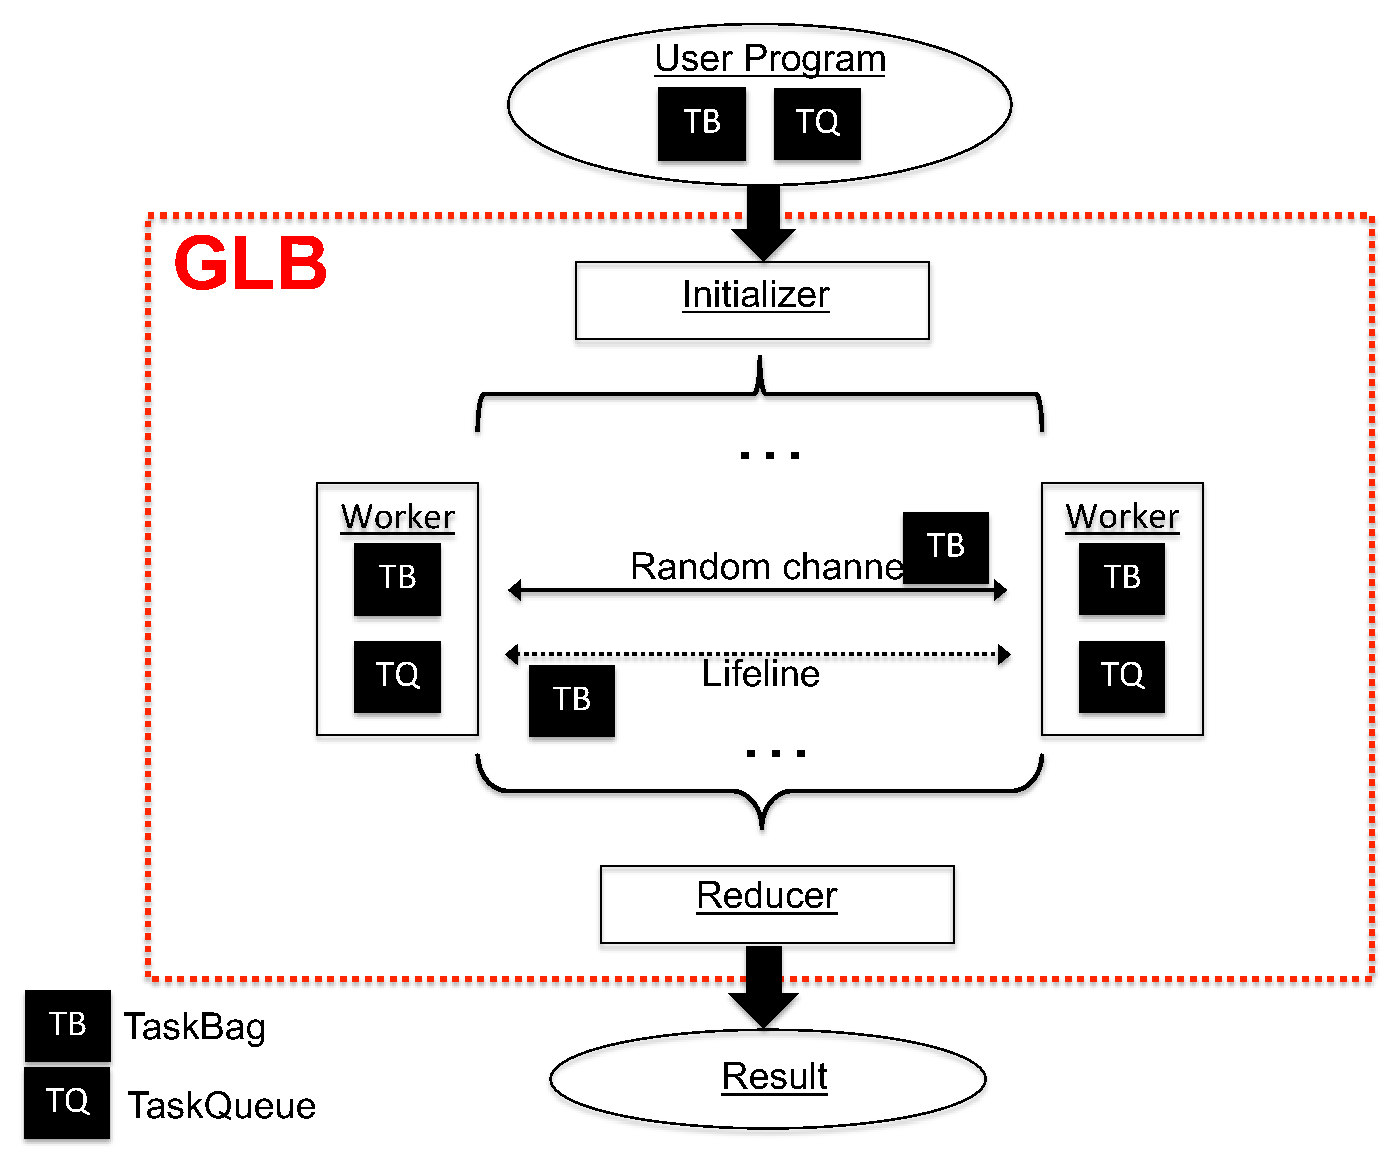
\includegraphics[width=3.25in]{./ppaa2014_figures/glb_overview.eps}
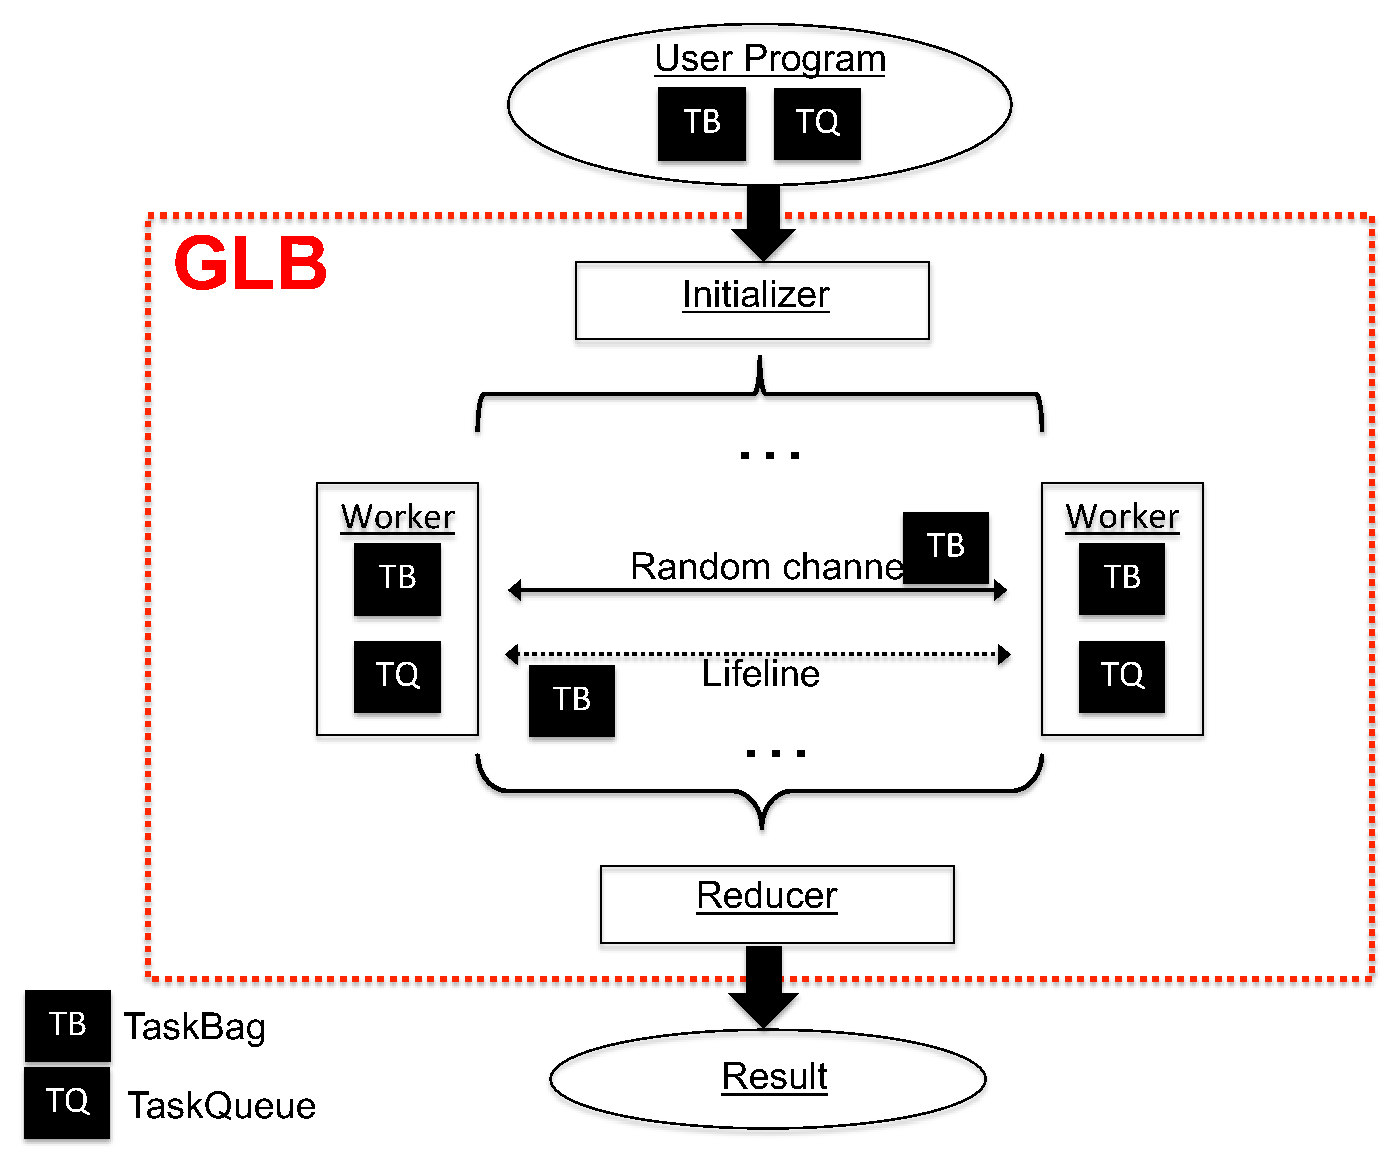
\includegraphics[scale=0.3]{./ppaa2014_figures/glb_overview.eps}
\caption{GLB overview}
\label{fig:design:glb}
\end{figure}


In the following sections, Section~\ref{sec:design:user} discusses what are required from users, Section~\ref{sec:design:internals} discusses the GLB internals, Section~\ref{sec:design:uts} discusses how to apply GLB to the UTS problem, Section~\ref{sec:design:bc} discusses how to apply GLB to the BC problem.


\subsection{What do users need to provide}
\label{sec:design:user}
\textbf{TaskQueue} Users need to provide an implementation of following methods:
\begin{enumerate}
\item \code{process(n:Long):Boolean} This method describes the sequential computation of the problem. It iterates over \textit{n} items in its TaskBag and computes each one of them. It processes $n$ items if available and returns true; otherwise it processes all available ($<n$) items and returns false. When GLB sees a Worker's process(n) returns false, it will schedule this Worker to steal from others.
 \item \code{split():TaskBag} Split its TaskBag and returns the split half. This method returns null if the TaskBag is too small to split.  
\item \code{merge(TaskBag)} Merge the incoming TaskBag to its own TaskBag.
Both split and merge method functions are wrapper functions that will call TaskBag's split/merge functions. 
\item \code{getResult()} Returns local result.
\item \code{reduce()} Result reduction function. Applying this function to each Worker's result yields the final result.
\end{enumerate}
\textbf{TaskBag} Users need to provide a custom class extending \textit{TaskBag} and appropriately implementing \code{split} and \code{merge} methods. They provide the functionalities that \textit{TaskQueue}'s \code{split/merge} methods need. GLB provides a default ArrayList-based TaskBag implementation. In this default implementation, split method is implemented by removing half of the elements from the end of the ArrayList and returning this removed half ArrayList; merge method is implemented by adding all the elements from the incoming ArrayList to the local ArrayList.  


Once the customized TaskQueue and TaskBag are implemented, it is fairly easy for
users to invoke GLB library by calling GLB's \code{run} method. If the workload cannot be statically scheduled across places, users need to provide an \code{initialize} method so that GLB will initialize this root task at place 0.  

\subsection{GLB internals}
\label{sec:design:internals}
GLB implements the lifeline work-stealing algorithm described in \cite{glb}. We summarize the algorithm here:
\begin{enumerate}
\item
Each Worker repeatedly calls \code{process(n)} method until it is running out of work. Between each process(n) call, Worker probes the network and responds to the stealing requests from other Workers. 
\item
When running out of work, a Worker conducts two rounds of work-stealing. It first chooses at most \textit{w} random victims. If none of the random victims has work to share, then Worker goes to the second round of work-stealing by stealing from its life-line buddies/victims. The topology of life-line communication graph is a $z$-dimensional hyper-cube. Such a topology satisfies these properties: it is a fully connected directed graph (so
work can flow from any vertex to any other vertex) and it has a low
diameter (so latency for work distribution is low) and has a low
degree (so the number of buddies potentially sending work to a dead
vertex is low). If a lifeline buddy cannot satisfy the stealing request due to its lack of work, it will still remember the request and try to satisfy the request when it gets work from others.   
\item
When all Workers run out of work, GLB terminates and applies the reduce function to each Worker's result to yield the final result.
\end{enumerate}

Users can tune the GLB performance by changing these parameters:
\textit{w}, \textit{z}, and \textit{n}. It is more likely to steal
work from a random victim with a larger $w$. It is more likely to
steal work from a lifeline buddy when $z$ is larger. However, when $w$
and $z$ get larger, each worker spends more time probing the network and less time in processing tasks. Alternatively, users can make a Worker spend more time on processing tasks by increasing $n$. The larger $n$ is, the more tasks a Worker needs to finish before it can respond to the stealing requests. However, a large $n$ can sometimes hurt the performance if stealing requests need be responded fast. We will see an extreme case in which even $n=1$ is too large a task-granularity in Section~\ref{sec:design:bc}.

To help users understand and tune GLB program performance, GLB also provides logging functionalities to record (1) how much time each Worker spent on processing and distributing work (2) how many (random/lifeline) stealing requests each Worker sent and received. (3) how many (random/lifeline) stealings each Worker perpetrated. (4) How much workload has each Worker received/sent.

To better illustrate how to use GLB, we show a pedagogical use case via the Fibonacci problem in the Appendix.



\subsection{UTS}
\label{sec:design:uts}
\subsubsection{Problem statement}
The Unbalanced Tree Search benchmark measures the rate of traversal of
a tree generated on the fly using a splittable random number
generator. For this submission, we used a \emph{fixed geometric law}
for the random number generator with branching factor $b_0=4$, seed
$r=19$, and tree depth $d$ varying from 13 to 20 depending on core counts and architecture.

\begin{quote}
The nodes in a geometric tree have a branching factor that follows a
geometric distribution with an expected value that is specified by the  
parameter $b_0 > 1$. The parameter $d$ specifies its maximum depth
cut-off, beyond which the tree is not allowed to grow ... The expected
size of these trees is $(b_0)^d$, but since the geometric distribution
has a long tail, some nodes will have significantly more than $b_0$
children, yielding unbalanced trees. 
\end{quote}

The depth cut-off makes it possible to estimate the size of the trees
and shoot for a target execution time. To be fair, the distance from
the root to a particular node is never used in our benchmark
implementation to predict the size of a subtree. In other words, all
nodes are treated equally, irrespective of the current depth.  

%% \subsubsection{Design}

%% The material in this section is excerpted from \cite{glb}, and
%% unchanged from our 2012 HPCC submission.

%% One common way to load balance is to use {\em work-stealing}. For
%% shared memory system this technique has been pioneered in the Cilk
%% system.  Each worker maintains a double ended queue (deque) of tasks. When a
%% worker encounters a new task, it pushes its continuation onto the
%% bottom of the deque, and descends into the task. On completion of the task, it
%% checks to see if its deque has any work, if so it pops a task (from the
%% bottom) and continues with the work. Else (its deque is empty) it
%% looks for work on other workers' deques. It randomly determines a {\em
%%   victim} worker, checks if its queue is non-empty, and if so, pops a
%% task from the top of the deque (the end other than the one being
%% operated on by the owner of the deque).  If the queue is empty, it
%% guesses again and continues until it finds work. Work-stealing systems
%% are optimized for the case in which the number of steals is much
%% smaller than the total amount of work. This is called the ``work
%% first'' principle -- the work of performing a steal is incurred by the
%% thief (which has no work), and not the victim (which is busy
%% performing its work). 

%% Distributed work-stealing must deal with some additional
%% complications. First, the cost of stealing is usually significantly
%% higher than in the shared memory case. For many systems, the target
%% CPU must be involved in processing a steal attempt. Additionally, one
%% must solve the distributed termination detection problem. The system
%% must detect when all workers have finished their work, and there is no
%% more work. At this point all workers should be shut down, and the
%% computation should terminate. 

%% X10 already offers a mechanism for distributed termination detection
%% -- \texttt{finish}. Thus, in principle it should be possible to spawn
%% an activity at each place, and let each look for work. To trigger
%% \texttt{finish} based termination detection however, these workers
%% must eventually terminate. But when? One simple idea is that a worker
%% should terminate after $k$ steal attempts have failed. However this
%% leaves open the possibility that a worker may terminate too early --
%% just because it happened to be unlucky in its first $k$ guesses. If
%% there is work somewhere else in the network then this work
%% can no longer be shared with these terminated workers, thereby
%% affecting parallel efficiency. (In an extreme case this could lead to
%% sequentialize significant portion of the work.) 

%% Therefore there must be a way by which a new activity can be launched 
%% at a place whose worker has already terminated. This leads to the idea
%% of a {\em lifeline graph}. For each place $p$ we pre-determine a set of
%% other places, called {\em buddies}. Once the worker at $p$ has
%% performed $k$ successive (unsuccessful) steals, it examines its
%% buddies in turn. At each buddy it determines whether there is some
%% work, and if so, steals a portion. However, if there is no work, it
%% records at the buddy that $p$ is waiting for work. If $p$ cannot find
%% any work after it has examined all its buddies, it dies -- the place $p$
%% now becomes quiescent.  

%% But if $P$ went to a buddy $B$, and $B$ did not have any work, then
%% it must itself be out looking for work -- hence it is possible that it
%% will soon acquire work. In this case we require that $B$ {\em
%%   distribute} a portion of the work to those workers that attempted to
%% buddy steal from it but failed. Work must be spawned on its own
%% \texttt{async} -- using the \texttt{at (p) async S} idiom. If $P$ had
%%  no activity left, it now will have a fresh activity. Thus, unlike
%%  pure work-stealing based systems, a system with lifeline graphs will
%%  see its nodes moving from a state of processing work (the active state), to a state in
%%  which they are stealing to a state in which they are dead, to a state
%%  (optionally) in which they are woken up again with more work (and are
%%  hence back in the active state).  

%% Note that when there is no work in the system, all places will be dead,
%% there will be no active \texttt{async} in the system and hence the
%% top-level \texttt{finish} can terminate. 

%% The only question left is to determine the assignment of buddies to a
%% place. We are looking for a directed graph that is fully connected (so
%% work can flow from any vertex to any other vertex) and that has a low
%% diameter (so latency for work distribution is low) and has a low
%% degree (so the number of buddies potentially sending work to a dead
%% vertex is low).  $z$-dimensional hyper-cubes  satisfy these properties
%% and have been implemented. 

%% \subsubsection{Implementation}\label{sec:uts-inline}
%% Our implementation follows from \cite{glb} and includes the
%% performance improvements described in our HPCC 2012 submission
%% (using \code{FINISH\_DENSE} to reduce the overhead of termination
%% detection), using \code{@Uncounted} asyncs,  and using a compact
%% representation of the active nodes in a place using an implicit (lower,
%% upper) bounds representation rather than an explicit enumeration.

%% We have made a change in how the native SHA1 code is integrated into
%% X10. Consequently we replaced all of the 169 lines of very complex C++ wrapper code
%% with 3 native annotations (i.e., 3 lines of C code embedded into X10) as for instance in:

%% {\small
%% \begin{verbatim}
%% def this(seed:Int, depth:Int) {
%%   @Native("c++", "rng_init((RNG_state*)this, seed);") {}
%%   this.depth = depth;
%% }
%% \end{verbatim}
%% }

%% We fixed a nasty deadlock condition when using multi-dimensional lifeline graphs.


%% \subsubsection{Verification}
%% The code was validated by checking the results for specific
%% configurations against pre-computed numbers. 


%% % Runs on MPI now ... were there any issues here?
%% \subsubsection{UTS-GLB}\label{sec:utsg}
%% UTS-G is a variant of UTS written using the GLB library. The code for
%% \code{GlobalLoadBalancer} and \code{LocalJobRunner} is no longer
%% needed, since they are part of the library. The code for managing bags
%% of tasks is refactored into a \code{UTSTaskBag} class. Similarly the
%% code for executing a UTS task \code{runATMostNTasks} in
%% \code{UTSTaskFrame} is similarly very straightforward.  The native
%% code (for SHA1 hashes) remains unchanged -- it belongs in the
%% application and not the library.

%% Thanks to the GLB library the number of X10 LOCs drops from 493 for UTS to 225 for UTS-G.

%% %% \subsection{Performance}
%% %% \begin{figure}
%% %% \centering
%% %% \includegraphics[width=3.25in]{figures/p7ih/uts-p7ih.eps}
%% %% \caption{X10 Performance for UTS (on Power~775)}
%% %% \label{fig:perf:uts-p7ih}

%% %% \includegraphics[width=3.25in]{figures/bgq/uts-bgq.eps}
%% %% \caption{X10 Performance for UTS (on Blue~Gene/Q)}
%% %% \label{fig:perf:uts-bgq}

%% %% \includegraphics[width=3.25in]{figures/k/uts-k.eps}
%% %% \caption{X10 Performance for UTS (on K)}
%% %% \label{fig:perf:uts-k}
%% %% \end{figure}

%% %% We report performance for UTS and UTS-G.

%% %% On Power~775, as we demonstrated in our 2012 HPCC Submission, UTS achieves linear speedup up to 50,000 cores. UTS-G is only marginally slower.

%% %% On Blue~Gene/Q and K however, we ran the code ``as is'' without having the time to tune the main parameters of the load balancer to the specifics of the architecture. These parameters include the mapping of the lifeline graph onto the network axes (especially the dimensionality) as well as the frequency of network probes. With proper tuning, we believe we can redress the curves dramatically. In essence, with our implementation and our 2012 runs at scale on Power~775, we established that the benchmark (for this family of trees at least) is compute bound.

%% %% On Blue~Gene/Q, the sequential performance of the UTS-G code is 15\% less than the UTS code: the higher-order implementation confuses the optimizer of the backend compiler (xlC). This is not the case on other platforms. As a result, UTS-G appears to scale better than UTS, but this is misleading.
%% %% At scale, they are more or less on par as UTS only achieves 60\% efficiency for now. Hence the sequential inefficiency of UTS-G can hide behind the latency of the load balancer.

%% %% The measurements on K are very preliminary. The code runs and computes correct results. The performance is under investigation.



%% %We discuss the performance together with UTS-G in Section~\ref{sec:utsg}.
%% %\todo{Performance analysis. Why are numbers bad for the K. Is
%% %  there some basic operation that is slow on the K?}

Clearly, UTS is a case that static load-balancing does not work.  Assume the sequential implementation of UTS is available (i.e., the code to grow the UTS tree and count the nodes), we now discuss how to apply GLB to it.
\subsubsection{UTS TaskBag and TaskQueue }
\textbf{UTS TaskBag} The internal representation of a UTS tree node is a triple(descriptor, low, high). Descriptor represents the hashed value of the node, low represents the smallest index of un-explored children, high represents the largest index of its un-explored children. The representation of a UTS tree is thus an array of UTS tree nodes.
 A UTS TaskBag is essentially a UTS tree. To split a UTS TaskBag, we evenly split each UTS node $n(d,l,h)$ to two nodes $n1(d,l,h1)$ and $n2(d,h2,h)$, where $h1$ and $h2$ are the middle points of $(l,h)$.  If none of the UTS tree node has more than one child node, then we do not split the tree, as it is cheaper to count the node locally than move it to a remote place and count it there. To merge a UTS TaskBag, we simply concatenate the incoming TaskBag's UTS node array to the local one.

\textbf{UTS TaskQueue} \code{process(n)} method counts at most $n$ UTS tree nodes. \code{reduce()} is a straightforward sum-reduction method on each place's UTS tree node count.

Finally, GLB initializes the workload by initializing the root UTS tree node at Place 0.

\subsection{BC}
\label{sec:design:bc}
\subsubsection{Problem statement}
% BC
The Betweenness Centrality benchmark is taken from the SSCA2 (Scalable
Synthetic Compact Application 2) v2.2 benchmark \cite{SSCA2};
specifically, we implement the ``fourth'' kernel in this benchmark,
the computation of {\em betweenness centrality}:

\begin{quotation}
The intent of this kernel is to identify the set of vertices in the
graph with the highest betweenness centrality score. Betweenness
Centrality is a shortest paths enumeration-based centrality
metric, introduced by Freeman (1977). This is done using a betweenness
centrality algorithm that computes this metric for every vertex in the
graph. Let $\sigma_{st}$ denote the number of shortest paths between
vertices $s$ and $t$, and $\sigma_{st}(v)$ the number of those paths
passing through $v$. Betweenness Centrality of a vertex $v$ is defined
as $BC(v) = \Sigma_{s\not=v\not=t \in V} \sigma_{st}(v)/\sigma_{st}$.

The output of this kernel is a betweenness centrality score for each
vertex in the graph and the set of vertices the highest betweenness
centrality score.
\end{quotation}

We implement the Brandes' algorithm described in the benchmark,
augmenting Dijkstra's single-source shortest paths (SSSP) algorithm,
for unweighted graphs. We have implemented the exact variant of the benchmark
(\code{K4approx=SCALE}). 

The solution we implement makes one very strong assumption: that the
graph is ``small'' enough to fit in the memory of a single
place. Since the graph itself is not modified during the execution of
this benchmark, it thus becomes possible to implement this benchmark
by replicating the graph across all places. Now effectively the
computation can be performed in an embarrassingly parallel fashion. The
set of $N$ vertices is statically partitioned among $P$ places; each place is
responsible for performing the computation for the {\em source}
vertices assigned to it (for all $N$ target vertices) and computes its
local \code{betweennessMap}. After this is
done an \code{allReduce} collective performs an \code{AND} summation
    across all local \code{betweennessMaps}. 

Clearly, statically partitioning the work amongst all places in this
way is possible but not ideal. The amount of work associated with one source node
$v$ vs another $w$ could be dramatically different. Consider for
instance a degenerate case: a graph of $N$ vertices, labeled $1\ldots
N$, with an edge $(i,j)$ if $i < j$. Clearly the work associated with
vertex $1$ is much more than the work associated with vertex $N$. 

We next discuss how to dynamically load-balance these
tasks across all places using the GLB framework. 

%% \subsubsection{Structure of the code}
%% The multi-place structure of this code is quite straightforward. We
%% use the standard at-scale X10 idiom for SPMD code:
%% \begin{enumerate}
%% \item Create a distributed data structure, accessed through a
%%   \code{PlaceLocalHandle} which points to an instance of a ``host''
%%   object (an instance of \code{SSCA2}) at each node. (Invocation of
%%   \code{makeFlat}.) 
%% \item Run the actual computation (invocation of \code{broadcastFlat}
%%   with the closure specifying the work to be done at each place.

%%   The work done in each place is the computation of a
%%   \code{bfsShortestPaths} for a slice of vertices from
%%   \code{startVertex} to \code{endVertex}. This loops through the
%%   vertices in the given range, computing the betweennessMap
%%   locally. 

%%   Note this computation is single threaded. It is not difficult to
%%   make this multi-threaded. 

%% \item Once the local computation has been done, and the local
%%   contribution to the betweennessMap computed, a
%%   \code{Team.WORLD.allreduce} ensures that the results are reduced and
%%   made available at place $0$. 
%% \end{enumerate}

%% \subsection{Validation.}
%% The benchmark calls for validating the algorithms by running it on a
%% graph (a torus)  with known analytical results for the betweenness
%% centrality.  Because of lack of time, we have not been able to do
%% this. If our submission is selected for presentation, we plan to
%% validate the algorithm by the time of the presentation.


%% \subsection{Performance measurement.}
%% We discuss the performance together with BC-G in Section~\ref{sec:bcg}.


\subsubsection{BC TaskBag and TaskQueue}
\textbf{TaskBag} Each vertex interval is a task item. We use a tuple(low, high) to represent a vertex interval. Each task bag is an array of such tuples. To split a TaskBag, we divide each tuple evenly. To merge a BC taskbag, we simply concatenate the incoming TaskBag's array to the local one.  

\textbf{TaskQueue} \code{process(n)}  method iterates over the taskbag and calculates the first n vertices. 
\textbf{reduce()} method is a simple betweenness-map (a vector) element-wise add function.

This implementation achieves linear speedup and perfect scalability on
small-scale machines (i.e., 256 cores on Power) for smaller
graph. However, it does not yield equally impressive performance on larger machines for larger graphs. After examining the GLB log, we realized that on large scale machines, Workers are less responsive to the stealing requests thus workload cannot be distributed fast. Therefore, we tried to maximize $w$ and $z$ and minimize $n$. (Please refer to Section~\ref{sec:design:internals} for the rationale of turning these parameters). The performance only improved slightly.
We then realized that it took a Worker too long before it responded to the work stealing requests even when its task granularity is \textbf{one} vertex. So we changed the code that computes each vertex to an interruptable state machine. In this way, a Worker can respond to stealing requests without completing one vertex computation. Alternatively, we can help users to minimize the code change by providing a yielding functionality in the GLB library. Users can insert yield points in the their code to increase its probing frequency and responsiveness to stealing requests. We plan to provide such functionality in GLB in the future work.


\section{Performance evaluation}
\subsection{Methodology}
\subsection{Unified code base}
We compare our GLB code to the legacy X10 implementation used to
evalutate X10 performance at Peta-scale~\cite{tardieu-petascale}. To
ensure a fair comparison, we use the same piece of sequential computation code for the legacy code and GLB code. 
\subsection{Platforms}
We evaluated the performance on 3 different architectures: Power~775,
Blue~Gene/Q, and K. We now briefly discuss each architecture and the compiler options we used.

%\subsection{Power~775}
\paragraph{Power-775}
We gathered performance results on a small Power~775 systems with two drawers.
A Power~775 octant (or host or compute node) is composed of a quad-chip module
containing four eight-core 3.84 Ghz Power7 processors, one optical
connect controller chip (codenamed {\em Torrent}), and 128 GB of
memory (in our current configuration). A single octant has a peak performance of 982 GFLOPS; a peak
memory bandwidth of 512 GB/s; and a peak bi-directional interconnect
bandwidth of 192 GB/s. %Each octant forms a single SMP node running an
operating system image. Eight octants are grouped together into a drawer.

Each octant runs RedHat Enterprise Linux 6.2 and uses IBM's PE MPI for network communication (over PAMI).  

We compiled the benchmark programs using Native X10 version 2.4.0 with \texttt{-NO\_CHECKS}, \texttt{-O} options, and compiled the resulting
C++ files with xlC 12.1 with the \texttt{-qinline} \texttt{-qhot} \texttt{-O3}
\texttt{-q64} \texttt{-qarch=auto} \texttt{-qtune=auto} compiler options.

We allocated 32 places per octant when we use multiple octants.
We used regular 64 KB pages for all the programs.


%\subsection{Blue~Gene/Q}
\paragraph{Blue~Gene/Q}
Our Blue~Gene/Q numbers were gathered on Vesta, a small Blue~Gene/Q
system located at Argonne National Laboratory.
Each compute node of the
Blue~Gene/Q is a 64-bit PowerPC A2 processor with 16 1.6 Ghz compute
cores and 16 GB of DRAM. The compute notes are grouped into drawers
(32 compute nodes per drawer), which are grouped into midplanes (16
compute drawers, 512 compute nodes).  Within the midplane, nodes are
electrically connected in a 5-D torus (4x4x4x4x2). Beyond the
midplane, an optical interconnect is used.  

All benchmarks were compiled using Native X10 version 2.4.0 with \texttt{-NO\_CHECKS}, \texttt{-O} options. The
generated C++ code was then compiled for Blue~Gene/Q using xlC v11.1
with
the \texttt{-O3} \texttt{-qinline} \texttt{-qhot} \texttt{-qtune=qp} \texttt{-qsimd=auto} \texttt{-qarch=qp}
command line arguments.

To maximize the number of X10 Places, all experiments with 16 Places or
more were run using the \texttt{c16} mode, which creates one MPI
process (i.e., one X10 Place) per Blue~Gene/Q compute core.  Thus each
X10 Place has 1 A2 core and 1 GB of DRAM available to it.  


%\subsection{K}
\paragraph{K}
The K computer is a supercomputer at RIKEN 
Advanced Institute for Computational Science.
It consists of 82944 compute nodes, and 
each node has one scalar CPU (SPARC64\textsuperscript{\texttrademark}VIIIfx, 8 cores, 128 GFLOPS)
and 16 GB memory.
These compute nodes are connected by Tofu interconnect,
which is 6D mesh/torus network having 10 links (5 GB/s x 2 bandwidth per link) on each node.

Each node runs Linux-based OS, and developers can use MPI-2.1 for network communication.

We compiled the benchmark programs using Native X10 version 2.4.0
with \texttt{-NO\_CHECKS}, \texttt{-O}, and \texttt{-FLATTEN\_EXPRESSIONS} options,
and compiled the resulting C++ files with Fujitsu C/C++ Compiler version K-1.2.0-14 
with \texttt{-Xg} and \texttt{-Kfast} options. 

We allocated 8 places per node when we use multiple compute nodes.
The memory page sizes were set as 32 MB for all the programs.




\subsection{Experimental results}
\subsection{UTS}
In this section, we demonstrate the UTS-GLB performance by showing
three figures, one per each architecture. On each architecture, we
compare the legacy code to the GLB implementation. One thing to note is that the legacy code is a highly tuned parallel implementation of UTS and it won the HPCC2012 performance award~\cite{tardieu-petascale}.
On each figure, the x-axis represents the number of places; the primary y-axis (the left y-axis) represents the number of UTS nodes counted per second; the secondary y-axis (the right y-axis) represents the efficiency, which is calculated by how many nodes counted per second per place. A straight line whose slope is 1 along the primary y-axis indicates a linear speedup and a horizontal line on the secondary y-axis indicates the implementation scales perfectly. In the following discussion, we refer to UTS legacy code by UTS and refer to UTS GLB code by UTS-G.

\begin{figure}
\centering
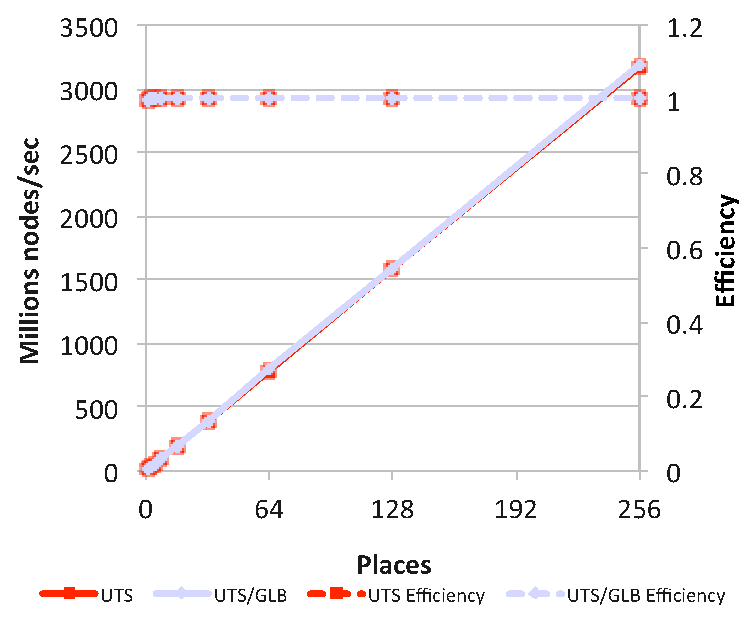
\includegraphics[width=2.25in]{./ppaa2014_figures/uts_p7ih.eps}
\caption{UTS/UTS-G Performance Comparison (on Power~775)}
\label{fig:perf:uts-p7ih}
\end{figure}

Figure ~\ref{fig:perf:uts-p7ih} shows the performance comparison for UTS and UTS-G on Power~775 up to 256 cores. UTS and UTS-G both achieve linear speedup and their efficiencies stay at 1, which means they both achieve perfect scaling.  

\begin{figure}
\centering
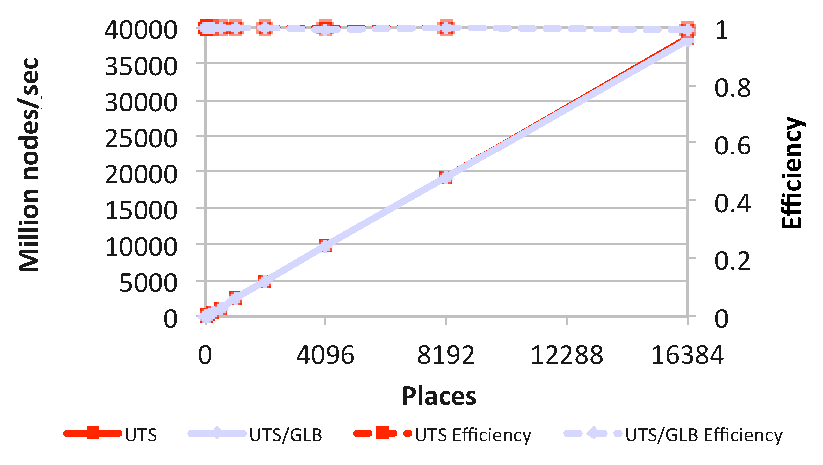
\includegraphics[width=2.55in]{./ppaa2014_figures/uts_bgq.eps}
\caption{UTS/UTS-G Performance Comparison (on Blue~Gene/Q)}
\label{fig:perf:uts-bgq}
\end{figure}
Figure ~\ref{fig:perf:uts-bgq} shows the performance comparison for UTS and UTS-G on Blue~Gene/Q up to 16384 cores. UTS and UTS-G both achieve linear speedup and perfect scaling. 

\begin{figure}
\centering
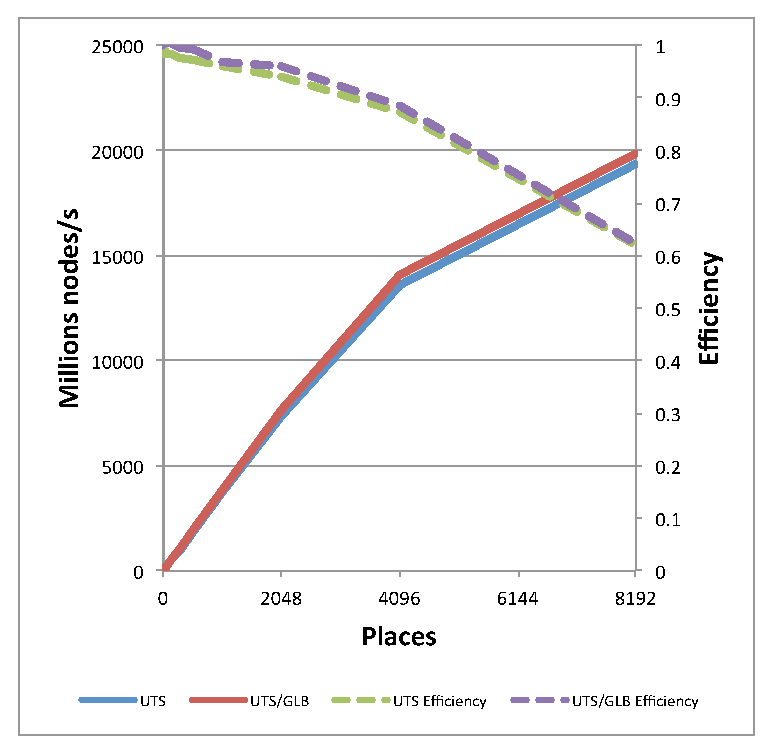
\includegraphics[scale=0.35]{./ppaa2014_figures/uts_k.eps}
\caption{UTS/UTS-G Performance Comparison  (on K)}
\label{fig:perf:uts-k}
\end{figure}
Figure ~\ref{fig:perf:uts-k} shows the performance comparison for UTS and UTS-G on Blue~Gene/Q up to 8192 cores. UTS and UTS-G perform well up to 4096 cores (i.e., almost linear speedup and efficiency stays above 0.9). When running on more than 4096 cores, both UTS and UTS-G drop their efficienies to 0.6. We are still investigating why there is a sudden performance drop on K.

\textbf{Summary} UTS-G achieves near linear speedup and perfect scaling on both Power~775 (up to 256 cores) and Blue~Gene/Q (up to 16384 cores). On all three architectures, UTS-G achieves similar (or better) performance compared to UTS, a highly tuned award-winning implementation.


\subsection{BC}
In this section, we compare the BC-GLB performance to the BC legacy
code. Two things to note are: (1) the legacy BC code uses a very
different synchronization scheme from the legacy UTS code. In
comparison, the GLB implementation of UTS and BC share exactly the
same synchronization scheme (i.e., the underlying GLB library). This
demonstrates GLB is applicable to widely different types of
problems. (2) The legacy BC implementation randomizes which vertices
to compute on each place, which effectively reduces the imbalance
among places. As the number of places increases, such imbalance
decreases. When running on more than 1024 places, BC's performance is
only roughly 15\% worse than then optimal performance (i.e., the longest execution time per place is only 15\% more than the average finishing time across all places). Therefore, it is difficult to improve the performance because the room to improve is limited. 

We demonstrate the UTS-GLB performance by showing six figures, two per each architecture. On each architecture, we first compare performance, then we compare the workload distribution among places.   
On each performance comparison figure, the x-axis represents the number of places; the primary y-axis (i.e., the left y-axis) represents the number of edges traversed per second; the secondary y-axis (i.e., the right y-axis) represents its efficiency, which is calculated by number of edges traversed per second per place. A straight line whose slope is 1 along the primary y-axis indicates a linear speedup and a horizontal line along the secondary y-axis indicates the implementation scales perfectly. To understand how effective GLB is at balancing the workload compared to the legacy code, we also plot the workload distribution graphs. On each workload distribution graph, we bar-plot the calculation time on each place and bundle them together. The more even workload distribution graph appears, the more balanced workload is. A rectangular visualization indicates the perfect load-balancing. We also show the mean and standard deviation of the workload distribution on each figure. In the following discussion, we refer to BC legacy code as BC and refer to BC-GLB code as BC-G. 

\begin{figure}
\centering
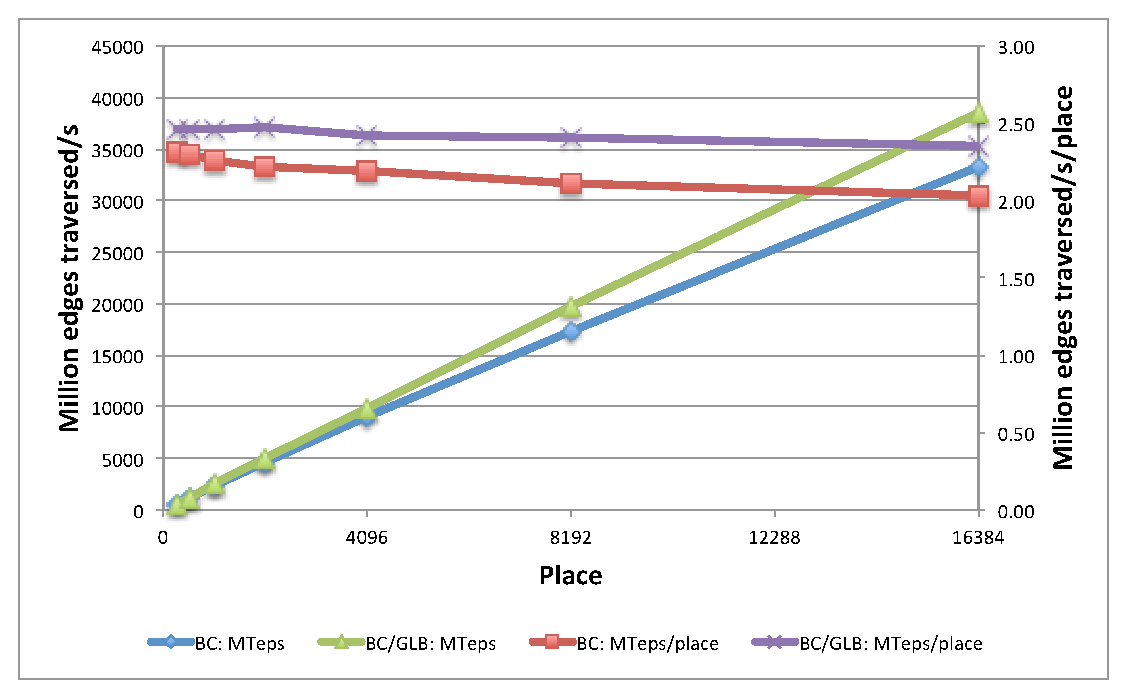
\includegraphics[width=2.25in]{./ppaa2014_figures/bc_bgq.eps}
\caption{BC/BC-G Performance (on Blue~Gene/Q)}
\label{fig:perf:bc-bgq}
\end{figure}
Figure~\ref{fig:perf:bc-bgq} shows the BC performance comparison on Blue~Gene/Q. We can see that GLB implementation achieves near linear speedup and near perfect scaling. 



\begin{figure}
\centering
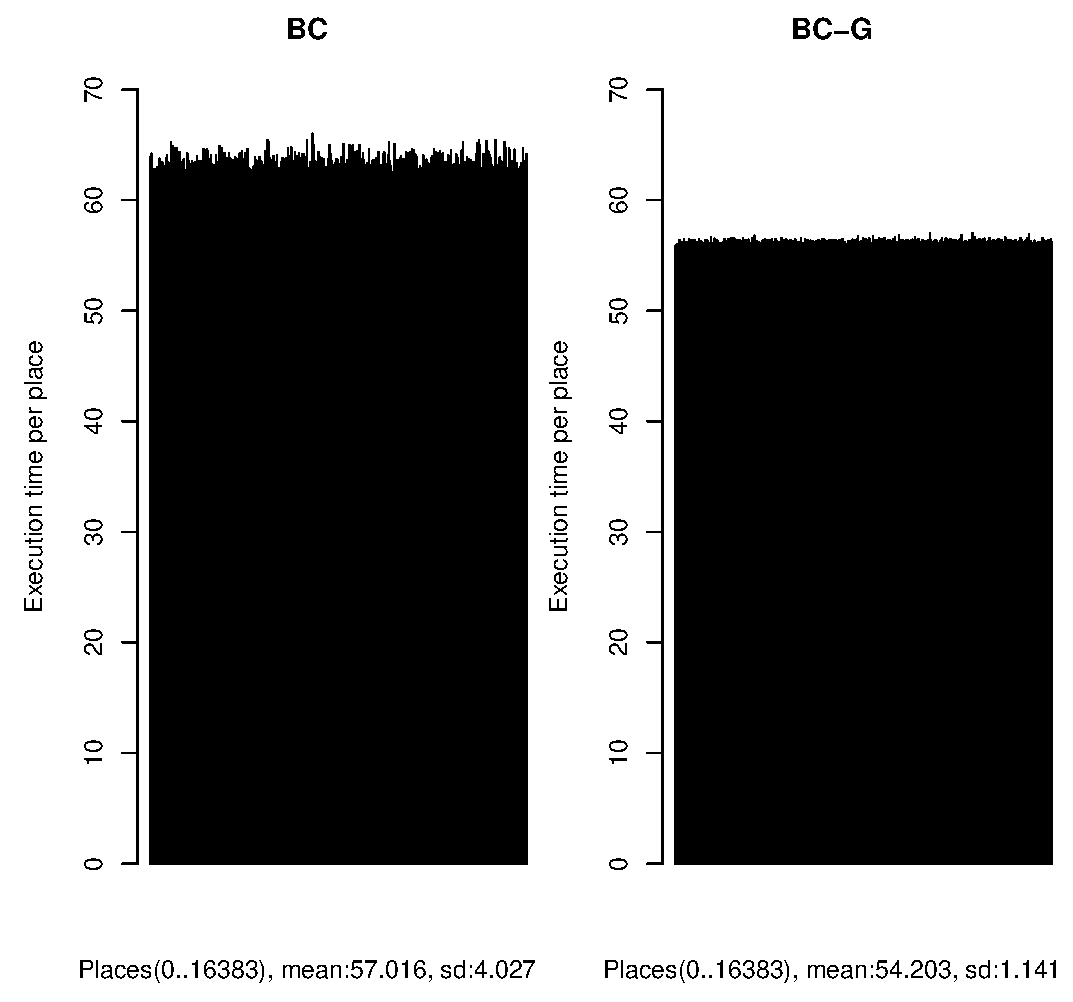
\includegraphics[width=2.25in]{./ppaa2014_figures/bgq_workload.eps}
\caption{BC/BC-G Workload Distribution (on Blue~Gene/Q)}
\label{fig:dist:bc-bgq}
\end{figure}
Figure~\ref{fig:dist:bc-bgq} shows the workload distribution of BC on Blue~Gene/Q. As we can see, BC-G workload distribution is much more even than that of BC, GLB reduces the standard deviation from 4.027 to 1.141. In fact, BC-G finishes calculation in 57.0586 seconds, which is almost equal to the mean of BC computing time accross all places (57.015s). This indicates that BC-G achieves the near perfect load-balancing on Blue~Gene/Q. 


\begin{figure}
\centering
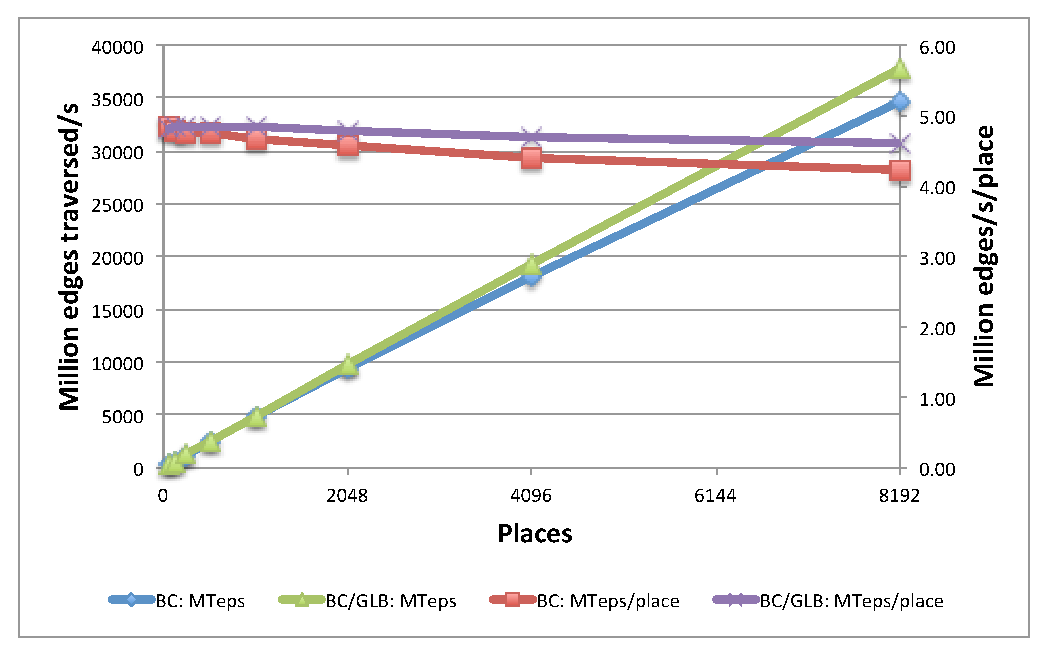
\includegraphics[width=2.25in]{./ppaa2014_figures/bc_k.eps}
\caption{BC/BC-G Performance (on K)}
\label{fig:perf:bc-k}
\end{figure}
Figure~\ref{fig:perf:bc-k} shows the BC performance comparison on K. BC-G also achieves near linear speedup and near perfect scaling (efficiency$>$0.95 up to 8192 places).


\begin{figure}
\centering
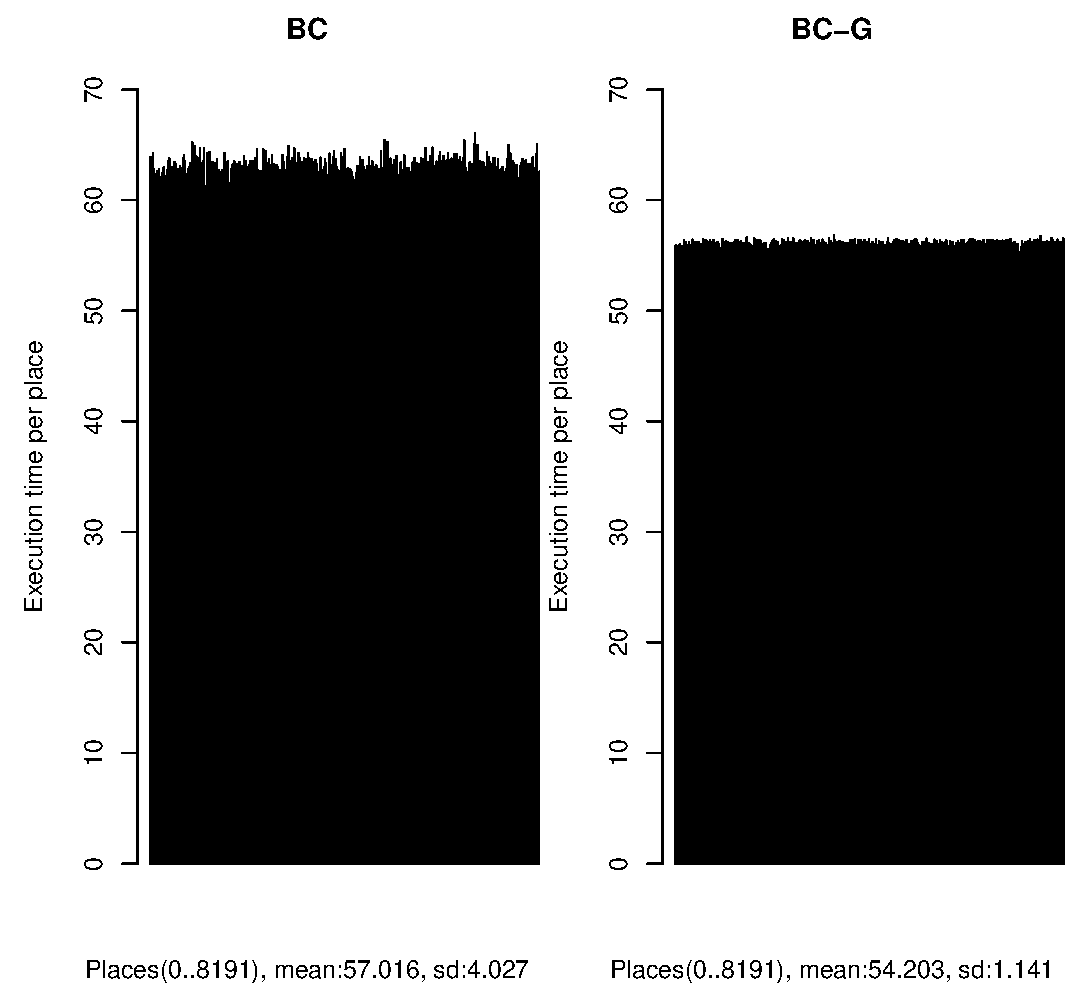
\includegraphics[width=2.25in]{./ppaa2014_figures/k_workload.eps}
\caption{BC/BC-G Workload Distribution (on K)}
\label{fig:dist:bc-k}
\end{figure}
Figure~\ref{fig:dist:bc-k} shows the workload distribution of BC on Blue~Gene/Q. As we can see, BC-G workload distribution is much more even than that of BC on K. BC-G finishes calculation in 58.198729 seconds on 8192 places, which is within 1.5\% of the mean of BC computing time across all places (57.016s). This indicates that BC-G also achieves the near perfect load-balancing on K. 


\begin{figure}
\centering
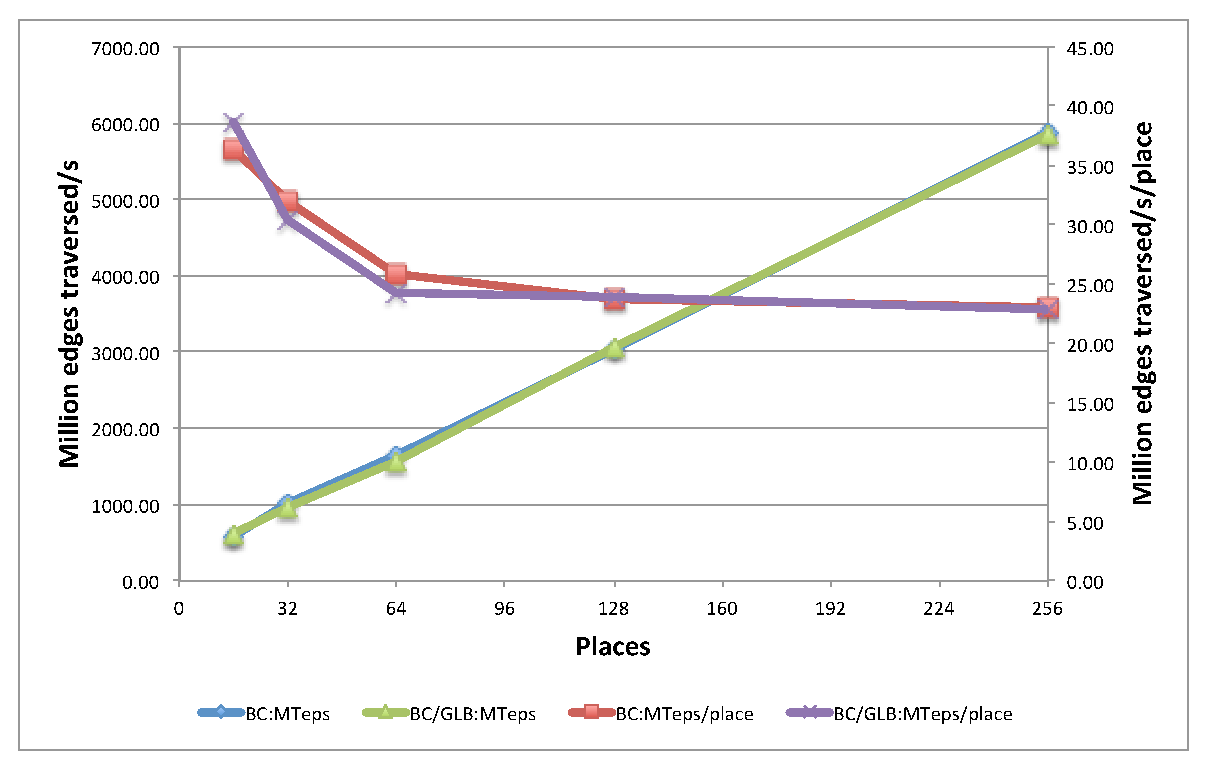
\includegraphics[width=2.25in]{./ppaa2014_figures/bc_p7ih.eps}
\caption{BC/BC-G Performance (on Power 775)}
\label{fig:perf:bc-p7ih}
\end{figure}
Figure~\ref{fig:perf:bc-p7ih} shows the BC performance comparison on
K. Surprisingly, BC-G on Power 775 does not achieve the linear speedup
and perfect scaling as it does on Blue~Gene/Q and on K. That is
because as the number of places increase, the total amount of time to
finish calculating all the vertices also increase even when the graph
stays the same.  Additionally, for the same workload, BC-G spends more
time calculating (on average 5-20\% more) than BC when both run on a
single place. We suspect both problems are due to the overly sensitive
C++ compiler optimizations on Power 755; we are still investigating to
verify this hunch. However, as demonstrated in Figure~\ref{fig:dist:bc-p7ih}, BC-G is very effective at removing the imbalance among workloads, it decreases the workload standard deviation from 58.463 to 1.482.
\begin{figure}
\centering
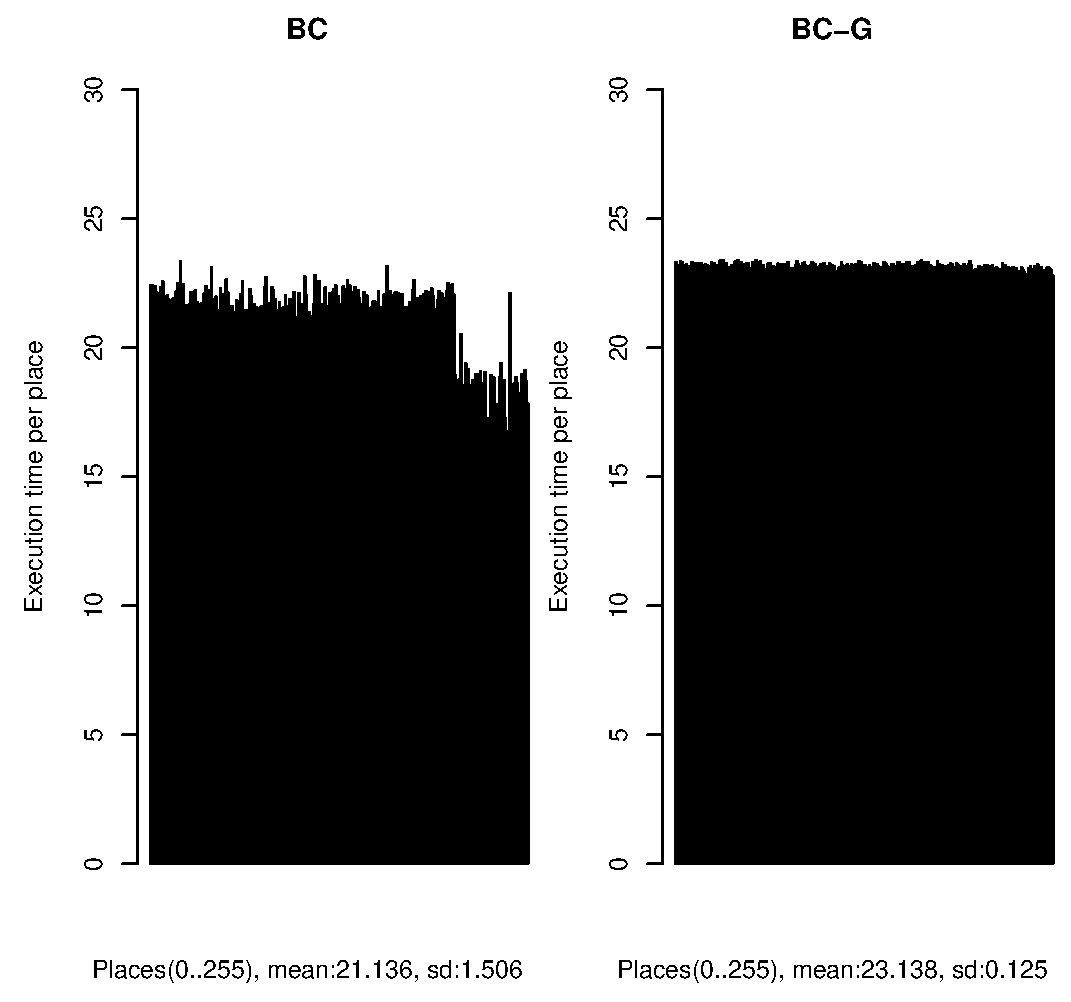
\includegraphics[width=2.25in]{./ppaa2014_figures/p7ih_workload.eps}
\caption{BC/BC-G Workload Distribution (on Power 775)}
\label{fig:dist:bc-p7ih}
\end{figure}

\textbf{Summary}  BC-G constantly outperforms the BC implementation. On Blue~Gene/Q (up to 16384 cores) and K (up to 8192 cores), BC-G achieves the near-optimal speedup, scalability and load-balancing.


\section{Future work}
We plan to do the following future work: 
(1) Investigate the performance anomaly of UTS-G on K and BC-G on Power 755.
(2) Provide yield points in the GLB library so that users can minimize the changes to the existing sequential code and improve the GLB program's responsiveness to work stealing requests.
(3) Experiment with more benchmarks.
(4) Provide a mechanism to auto-tune GLB parameters (e.g., task granularity, size of random victims/lifeline buddies).



\section{Related work}

There is extensive prior work on dynamic load balancing for
shared-memory systems.  The Cilk~\cite{FrigoLeRa98} system was the
first to provide efficient load balancing for a wide variety of
irregular applications.  Load balancing in Cilk applications is
achieved by a scheduler that follows the \textit{depth-first work,
  breadth-first steal} principle~\cite{blumofe:94}. Cilk's scheduling
strategy, in which each worker maintains its own set of
tasks and steals from other workers when it has nothing to do, is
often referred to as \textit{work-stealing}.  
%
Following Cilk, many runtimes for shared memory task parallelism
utilize work-stealing schedulers. 
%
Of these, OpenMP 3.0~\cite{openmp30:08}, Intel's Threading
Building Blocks (TBB)~\cite{reinders:07}, 
Java Fork-Join~\cite{DL2000}, Microsoft's Parallel Patterns
Library (PPL), and Task Parallel Library (TPL) are the most popular.
% Several implementations of X10's async-finish programming model have
utilized work-stealing schedulers including X10's
\textit{breadth-first}~\cite{cong:08} and
\textit{compiler-supported}~\cite{TOWH2012} and Guo et
al.'s~\cite{sarkar:09} hybrid model for work stealing.

The techniques for dynamic load balancing in shared-memory
environments are not directly applicable to distributed-memory
machines because of a variety of issues such as network latency and
bandwidth, and termination detection. 
%
Various bodies of work have addressed the problem of dynamic load balancing on
distributed-memory machines.
% 
Grama et al.~\cite{vipin:94,grama:99} discuss various load balancing 
strategies for distributed parallel searches that are independent of the 
specific search technique.
%
Blumofe et al.~\cite{blumofe:97} adapt the Cilk work-stealing model to 
distributed shared memory by limiting the scope of the programs to be purely 
functional.
%
ATLAS~\cite{baldeschwieler:96} and Satin~\cite{nieuwport:01} both use 
hierarchical work-steal to acheive global load balancing.
%
\Charmpp{}~\cite{sinha:93,kale:93} monitors the execution of its distributed
programs for load imbalance and migrates computation objects to low-load places
to correct the load imbalance.
%
Global load balancing for message passing environments has been researched 
for specific problems by Batoukov and Sorevik~\cite{batoukov:99}.

UTS, an excellent example of an irregular application, was first described by
Prins et al.~\cite{prins:03}.  It has since been widely used as a
benchmark for dynamic load balancing. 
%
Olivier and Prins~\cite{olivier:08} provided the first scalable implementation
of UTS on clusters that provided up to 80\% efficiency on 1024 nodes.
%
To this end, they employed a custom application-level load balancer along with
optimizations such as one-sided communications and novel termination detection
techniques.
% 
Dinan et al.~\cite{dinan:09} provide a framework for
global load balancing, which was used to achieve speedups on UTS on 8196
processors. Global load balancing and termination detection facilities
were provided to express irregular applications.
%
By reserving one core per compute node on the cluster exclusively for lock and
unlock operations, this framework allowed threads to steal work asynchronously
without disrupting the victim threads. However, the cost paid was a static
allocation (one core out of every eight) for communication. This results in
lower throughput because the thread is not available for user-level
computations.
% 
Saraswat et al.~\cite{glb} introduced lifeline-based global load
balancing and showed 87\% efficiency on 2048 nodes. Later work by the
X10 team demonstrated 98\% parallel efficiency with 55,680 Power7
cores~\cite{tardieu-petascale}.  An implementation of the life-line
algorithm in Co-Array Fortran achieved 58\% efficiency at 8192
nodes~\cite{CAF-HPCC2011}. A more recent UTS code using CAF 2.0 {\tt
  finish} construct achieves a 74\% parallel efficiency on 32,768
Jaguar cores~\cite{Chaoran:2013}.

%% Dave: Leaving this point out since we're tight on space and short
%%  on time...
%
% More broadly, the approach to programming taken by our GLB library
% in which the end-user of a framework provides snippets of
%sequential code that mesh with an underlying distributed framework is
% a commonly applied paradigm. Systems such as J2EE and MapReduce...


 


\section*{Acknowledgments}
The code for BC was developed in collaboration with Anju
Kambadur. Earlier versions of the code presented here were worked on
by Sreedhar Kodali, Ganesh Bikshandi, David Cunningham, Pradeep Varma,
Krishna Venkat and other colleagues.  

This material is based upon work supported by the Defense Advanced
Research Projects Agency under its Agreement No.~HR0011-07-9-0002, 
by the Department of Energy and by the Air Force Office of Scientific
Research. 

Some of the results were obtained by using the K computer at the RIKEN
Advanced Institute for Computational Science.  This research was
partially supported by JST, CREST.

This research used resources of the Argonne Leadership Computing
Facility at Argonne National Laboratory, which is supported by the
Office of Science of the U.S. Department of Energy under contract
DE-AC02-06CH11357.

\bibliographystyle{abbrv}
\bibliography{x10}

%\appendix
%\section{Selected Code Fragments}
\begin{appendices}
%% \subsection{A pedagogical use case via Fibonacci}
%% \label{sec:design:fib}
\begin{figure}
  \centering
   \mbox{\lstinputlisting[numbers=left, mathescape,basicstyle=\ttfamily\tiny, firstline=1, lastline=100]{./ppaa2014_figures/fib.java}}
   \caption{GLB-Fibonacci example}
  \label{fig:design:fib}
\end{figure}
We demonstrate how to use GLB via a Fibonacci example. We show the complete code in Figure~\ref{fig:design:fib}. 
Specifically, We apply GLB to Fibonacci($n$) in the following way: 
\begin{enumerate}
\item \textit{TaskBag} We use the default GLB Arraylist-based Taskbag, as shown at line 3. A task is an integer $i$ whose Fibonacci number should be computed. One can split/merge the TaskBag by calling the \code{merge} and \code{split} methods in the default TaskBag, as shown in Line22 -- Line 27. 
\item \textit{TaskQueue} Each TaskQueue keeps a $result$ of Long type, as shown at line 4.  To process each task item $i$, we first judge if it is less than 2, if so, add $i$ to $result$; if not, remove $i$ from the TaskBag and add $i-1$ and $i-2$ to the TaskBag. When its TaskBag becomes empty, TaskQueue's $result$ is the Fibonacci number of $n$. The \code{process} method is shown in line 10 -- line 21. The reduce function is a simple add function, as shown in line 28  -- line 30. 
\item \textit{Invoke GLB} Since it is difficult to statically schedule tasks among places for the Fibonacci problem, users can invoke GLB by calling the \code{run} method with an \code{initialize} method to use at the root place, as shown in line 35 and line 36. Were it easy to statically load balance, users could call the \code{run} method without providing the initialization method. 
\end{enumerate} 

Note that only these three pieces of code are required from the users and users are oblivious to any synchronization mechanism in X10. 

\end{appendices}
\end{document}
